\documentclass{article}
\usepackage{graphicx}
\usepackage{amsmath}

\begin{document}

\title{New York University \\ Tandon School of Engineering \\ Department of Computer Science and Engineering \\ Introduction to Operating Systems \\ Fall 2024 \\ Assignment 4 (10 points)}
\maketitle

\section*{Problem 1 (2 points)}

If you create a main() routine that calls fork() twice, i.e., if it includes the following code:

\texttt{pid\_t x=-11, y=-22;} \\
\texttt{x = fork();}\\
\texttt{if(x==0) y = fork(); }

Assuming all fork() calls succeed, draw a process tree similar to that of Fig. 3.8 (page 116) in your textbook, clearly indicating the values of x and y for each process in the tree (i.e., whether 0, -11, -22, or larger than 0). Note that the process tree should only have one node for each process and thus the number of nodes should be equal to the number of processes. The process tree should be a snapshot just after all forks completed but before any process exists. Each line/arrow in the process tree diagram shall represent a creation of a process, or alternatively a parent/child relationship.

\textbf{Process Tree Diagram:}

\begin{center}
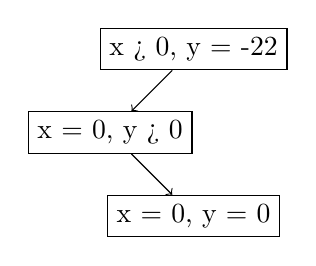
\begin{tikzpicture}[node distance=1.5cm]
  \node (A) [rectangle, draw] {x > 0, y = -22};
  \node (B) [rectangle, draw, below left of=A] {x = 0, y > 0};
  \node (C) [rectangle, draw, below right of=B] {x = 0, y = 0};
  \draw [->] (A) -- (B);
  \draw [->] (B) -- (C);
\end{tikzpicture}
\end{center}


\section*{Problem 2 (4 points)}

Write a program that creates the process tree shown below:

\textbf{Process Tree Diagram:}  (Same as Problem 1's diagram)

\texttt{
#include <stdio.h>
#include <unistd.h>
#include <sys/types.h>

int main() {
  pid_t x, y;
  x = fork();
  if (x == 0) {
    y = fork();
    if (y == 0) {
      printf("Process x=0, y=0\n");
    } else {
      printf("Process x=0, y>0\n");
    }
  } else {
    printf("Process x>0, y=-22\n");
  }
  return 0;
}
}
}
}
}
}

\section*{Problem 3 (4 points)}

Write a program whose main routine obtains a parameter n from the command line (i.e., passed to your program when it was invoked from the shell, n>2) and creates a child process. The child process shall then create and print a Fibonacci sequence of length n and whose elements are of type \texttt{unsigned long long}. The parent waits for the child to exit and then prints two additional Fibonacci elements, i.e., the total number of Fibonacci elements printed by the child and the parent is n+2. Do not use IPC in your solution to this problem (i.e., neither shared memory nor message passing).


\texttt{
#include <stdio.h>
#include <stdlib.h>
#include <unistd.h>
#include <sys/wait.h>

int main(int argc, char *argv[]) {
  if (argc != 2) {
    fprintf(stderr, "Usage: %s <n>\n", argv[0]);
    return 1;
  }

  long long n = atoll(argv[1]);
  if (n <= 2) {
    fprintf(stderr, "n must be greater than 2\n");
    return 1;
  }

  pid_t pid = fork();

  if (pid == 0) { // Child process
    unsigned long long a = 0, b = 1, temp;
    printf("Fibonacci sequence (child): ");
    for (long long i = 0; i < n; i++) {
      printf("%llu ", a);
      temp = a + b;
      a = b;
      b = temp;
    }
    printf("\n");
    exit(0);
  } else if (pid > 0) { // Parent process
    wait(NULL);
    unsigned long long a = 0, b = 1, temp;
    for (int i = 0; i < 2; i++) {
        temp = a + b;
        a = b;
        b = temp;
    }
    printf("Fibonacci sequence (parent): %llu %llu\n", a, b);
  } else {
    perror("fork");
    return 1;
  }

  return 0;
}
}

\section*{What to hand in (using Brightspace):}

Please submit the following files individually:

1) Source file(s) with appropriate comments. The naming should be similar to “lab\#\_\$.c” (\# is replaced with the assignment number and \$ with the question number within the assignment, e.g., \texttt{lab4\_b.c}, for lab 4, question b OR \texttt{lab5\_1a} for lab 5, question 1a).

2) A single pdf file (for images + report/answers to short-answer questions), named “lab\#.pdf” (\# is replaced by the assignment number), containing:
    \begin{itemize}
        \item Screenshot(s) of your terminal window showing the current directory, the command used to compile your program, the command used to run your program, and the output of your program.
    \end{itemize}

3) Your Makefile, if any. This is applicable only to kernel modules.


\section*{RULES:}

\begin{itemize}
    \item You shall use kernel version 4.x.x or above. You shall not use kernel version 3.x.x.
    \item You may consult with other students about GENERAL concepts or methods but copying code (or code fragments) or algorithms is NOT ALLOWED and is considered cheating (whether copied from other students, the internet, or any other source).
    \item If you are having trouble, please ask your teaching assistant for help.
    \item You must submit your assignment prior to the deadline.
\end{itemize}

\vspace{1cm}
\textbf{Note:}  The LaTeX code above provides a framework. You will need to add the process tree diagrams and the code solutions for parts A, B, and C.  The included HTML is largely irrelevant to the assignment itself and was omitted for clarity.  The  exam questions from the included HTML would need to be added as a separate section if desired.
\end{document}